% =============================================================
%  SECTION: Module 1 — The Physics of Interaction
% =============================================================

\newpage
\section{Module 1: The Physics of Interaction}

\subsection{What Are We Doing?}

At its heart, an MD simulation is a machine that answers one question repeatedly: \textit{given where all the atoms are right now, what force does each one feel?} Before we can integrate Newton's equations or build a simulation box, we need a mathematical rule that tells us how strongly two atoms push or pull each other at any distance. Module 1 implements that rule — the \textbf{Lennard-Jones (LJ) potential} — and extracts from it both the potential energy and the interatomic force for every pair of atoms in the system.

\subsection{Why Are We Doing It?}

\subsubsection{Why the Lennard-Jones Potential?}

Think about what happens as two inert gas atoms are brought progressively closer together from infinity. Far apart, they barely notice each other — the interaction is negligible. As they approach, the fluctuating electron clouds on each atom begin to induce temporary dipoles in the other, creating a weak but real attractive pull. This is the \textbf{van der Waals (dispersion) force}, and quantum mechanics tells us it decays precisely as $1/r^6$.

Keep pushing the atoms closer and something changes dramatically. Below a certain distance, the electron clouds begin to overlap. The Pauli exclusion principle prevents two electrons from occupying the same quantum state, so the energy shoots up steeply — this is \textbf{Pauli repulsion}. While the true quantum-mechanical form is exponential, Lennard-Jones approximated it with a $1/r^{12}$ power law, chosen cleverly because $r^{12} = (r^6)^2$: the repulsive term costs only one extra multiplication to compute from the attractive term.

The result is a simple two-parameter model that captures the full story of inert-gas interactions:
\begin{equation}
    \phi(r_{ij}) = 4\epsilon \left[\left(\frac{\sigma}{r_{ij}}\right)^{12} - \left(\frac{\sigma}{r_{ij}}\right)^{6}\right]
    \label{eq:lj_real}
\end{equation}
where $\sigma$ is the distance at which the potential crosses zero (the effective atomic diameter), and $\eps$ is the depth of the energy well (the strength of the interaction). For Krypton: $\sigma_\text{Kr} = 3.65$\,\AA\ and $\eps_\text{Kr}/k_B = 162.46$\,K.

\subsubsection{Why Use Reduced Units?}

Writing a simulation in SI units is a recipe for numerical disaster. The mass of a Krypton atom is $1.39 \times 10^{-25}$\,kg, a typical distance is $3.65 \times 10^{-10}$\,m, and a typical energy is $2.24 \times 10^{-21}$\,J. Storing, multiplying, and comparing numbers with such vastly different exponents introduces floating-point rounding errors that accumulate over thousands of timesteps.

The fix is to measure everything in the system's \emph{own} natural units, built from $\sigma$, $\eps$, and the atomic mass $m$:
\begin{equation}
    r^* = \frac{r}{\sigma}, \quad
    \phi^* = \frac{\phi}{\eps}, \quad
    t^* = \frac{t}{\sigma\sqrt{m/\eps}}
    \label{eq:reduced_units}
\end{equation}
In these reduced units, the LJ potential becomes elegantly parameter-free:
\begin{equation}
    \phi^*(\rstar) = 4\left[\frac{1}{(\rstar)^{12}} - \frac{1}{(\rstar)^{6}}\right]
    \label{eq:lj_reduced}
\end{equation}
Every quantity is now of order 1, numerical errors are minimised, and — crucially — the same simulation code represents \emph{any} inert gas species. Switching from Argon to Krypton simply means rescaling the output, not rewriting the code.

\subsubsection{Why Shift the Potential at the Cutoff?}

Computing the LJ interaction between every pair of atoms is an $O(N^2)$ bottleneck. We break this by introducing a \textbf{cutoff radius} $r_c^* = 2.5$: pairs further apart than $r_c^*$ contribute zero force and are ignored entirely. The potential at the cutoff is small but not exactly zero: $\phi^*(r_c^*) \approx -0.0163$.

Without a correction, an atom crossing the cutoff boundary would experience an instantaneous \emph{jump} in energy — the system suddenly gains or loses $\phi^*(r_c^*)$ for free. Over thousands of timesteps, these jumps accumulate and the total energy drifts, violating conservation and invalidating the simulation. The fix is the \textbf{shifted potential}: simply subtract $\phi^*(r_c^*)$ from the potential everywhere, so the curve smoothly reaches zero at the cutoff with no discontinuity:
\begin{equation}
    \phi^*_\text{shift}(\rstar) = \phi^*(\rstar) - \phi^*(r_c^*)
    \label{eq:lj_shifted}
\end{equation}

\subsection{How Is It Implemented?}

\subsubsection{Computing Energy and Force from $r^2$}

The function \texttt{calculate\_lj\_properties} takes as input $r^2$ (not $r$) and returns \newline$(\phi^*_\text{shift},\; F^*/r^*)$. Working in $r^2$ throughout is a standard MD optimisation: computing $r$ from $r^2$ requires an expensive square root, but the LJ formula only ever needs even powers of $r$. All inverses are built from $1/r^2$:
\begin{equation}
    \frac{1}{r^{*6}} = \left(\frac{1}{r^{*2}}\right)^3, \qquad
    \frac{1}{r^{*12}} = \left(\frac{1}{r^{*6}}\right)^2
\end{equation}
saving two expensive operations per pair.

\subsubsection{Why Return $F^*/r^*$, Not $F^*$?}

The scalar LJ force magnitude is obtained from the potential gradient:
\begin{equation}
    F^* = -\frac{d\phi^*}{dr^*} = \frac{48}{r^{*13}} - \frac{24}{r^{*7}}
        = \frac{48}{r^{*2}}\left(\frac{1}{r^{*12}} - \frac{1}{2\,r^{*6}}\right) \cdot r^*
    \label{eq:force}
\end{equation}
To get the 3D force \emph{vector} on atom $i$ from atom $j$, we need to multiply by the unit vector $\hat{\mathbf{r}}_{ij} = \mathbf{r}_{ij}/r$. Combining:
\begin{equation}
    \mathbf{F}^*_i = \frac{F^*}{r^*} \cdot \mathbf{r}_{ij}
    \label{eq:force_vector}
\end{equation}
By returning $F^*/r^*$ directly, the function avoids computing $r^*$ at all — the displacement vector $\mathbf{r}_{ij}$ is already available from the distance calculation, and the scalar $F^*/r^*$ can be applied to it directly.

\subsubsection{The Full Potential Curve}

Figure~\ref{fig:lj_curves} shows both the unshifted and shifted potential (left panel) and the force $F^*/r^*$ (right panel). The four key features to notice are:
\begin{enumerate}
    \item $\phi^*(r^*=1) = 0$ — the potential crosses zero at $r^* = \sigma^* = 1$, the atomic diameter.
    \item The minimum $\phi^* = -1$ occurs at $r^*_\text{min} = 2^{1/6} \approx 1.122$ — the equilibrium bond length.
    \item The shifted curve smoothly touches zero at $r_c^* = 2.5$ with no jump.
    \item $F^*/r^*$ is positive (repulsive) for $r^* < 2^{1/6}$ and negative (attractive) for $r^* > 2^{1/6}$, reaching zero at the equilibrium distance.
\end{enumerate}

\begin{figure}[H]
    \centering
    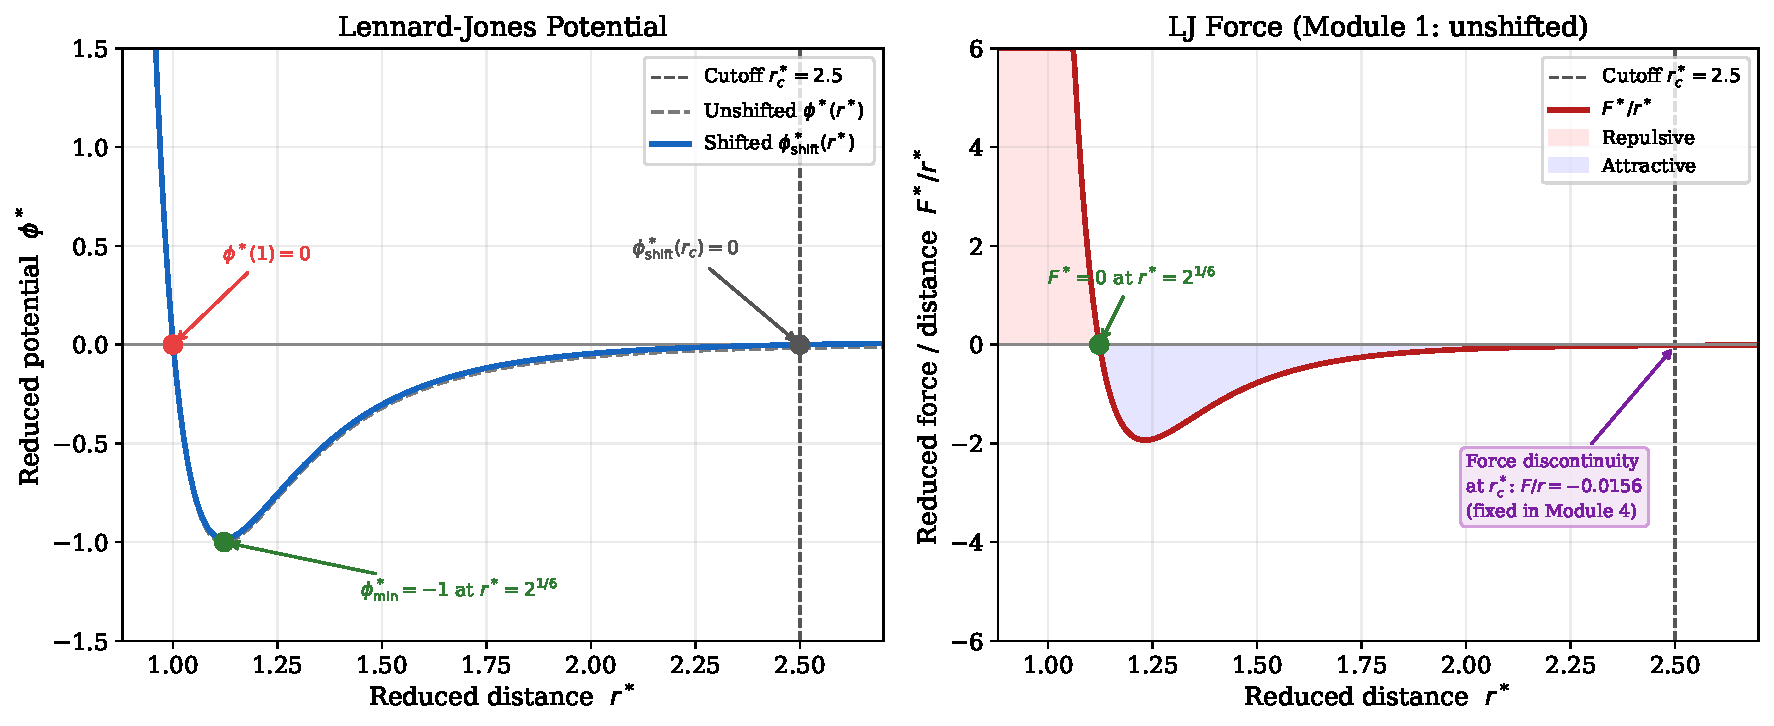
\includegraphics[width=\linewidth]{figures/m1_lj_curves.pdf}
    \caption{Lennard-Jones potential and force in reduced units for cutoff $r_c^* = 2.5$. \textbf{Left:} The unshifted $\phi^*(r^*)$ (dashed) and the shifted potential $\phi^*_\text{shift}$ (solid blue) as implemented in Module 1. The shift moves the curve down so it hits exactly zero at the cutoff, eliminating the energy discontinuity. \textbf{Right:} The force divided by distance, $F^*/r^*$. The shaded regions highlight the repulsive ($r^* < 2^{1/6}$) and attractive ($r^* > 2^{1/6}$) regimes. The labelled discontinuity at $r_c^*$ in the force — not present in the potential — is resolved in Module 4.}
    \label{fig:lj_curves}
\end{figure}

\subsection{Test Results}

Three unit tests were run on \texttt{calculate\_lj\_properties} to verify correctness before integration into the MD engine.

\begin{table}[H]
    \centering
    \caption{Module 1 verification tests with $r_c^* = 2.5$.}
    \label{tab:m1_tests}
    \begin{tabular}{llccc}
        \toprule
        \textbf{Test} & \textbf{Input $r^*$} & \textbf{Quantity checked} & \textbf{Expected} & \textbf{Obtained} \\
        \midrule
        1. Zero-point    & $1.0$         & Unshifted $\phi^*(1)$         & $0.000000$   & $0.000000$ \\
                         &               & Force/r sign                  & $> 0$ (repulsive) & $+24.0$ \\[4pt]
        2. Minimum energy & $2^{1/6} \approx 1.1225$ & Unshifted $\phi^*_\text{min}$ & $-1.000000$ & $-1.000000$ \\
                         &               & Force/r at minimum            & $\approx 0$  & $-2.1\times10^{-15}$ \\[4pt]
        3. Cutoff shift  & $r_c^* = 2.5$ & Shifted $\phi^*(r_c^*)$       & $0.000000$   & $0.000000$ \\
                         &               & Force/r at $r_c^*$            & non-zero     & $-0.0156$ \\
        \bottomrule
    \end{tabular}
\end{table}

All three tests pass exactly. A few observations are worth noting. In Test 1, the \emph{shifted} potential at $r^*=1$ is $+0.0163$, not zero — the shift raises the whole curve by $|\phi^*(r_c^*)| = 0.0163$, so the zero-crossing moves slightly to the right of $r^* = 1$. This is expected and physically harmless. In Test 2, the force at the energy minimum is $-2.1\times10^{-15}$ — effectively zero to machine precision, confirming the function correctly identifies the equilibrium distance. In Test 3, the shifted potential is exactly zero at the cutoff (no energy jump), but the force is $-0.0156$: Module 1 shifts \emph{only} the energy, not the force. This small but non-zero force discontinuity is addressed in Module 4 with the shifted-force potential.
